\begin{center} [\textit{Teil 2}]
\end{center}
\pend
%\vspace{0,5em}
\count\Bfootins=1200
\count\Cfootins=1200
\pstart
\noindent
%\begin{wrapfigure}[13]{l}{0.46\textwidth}
%\vspace{-11pt}
%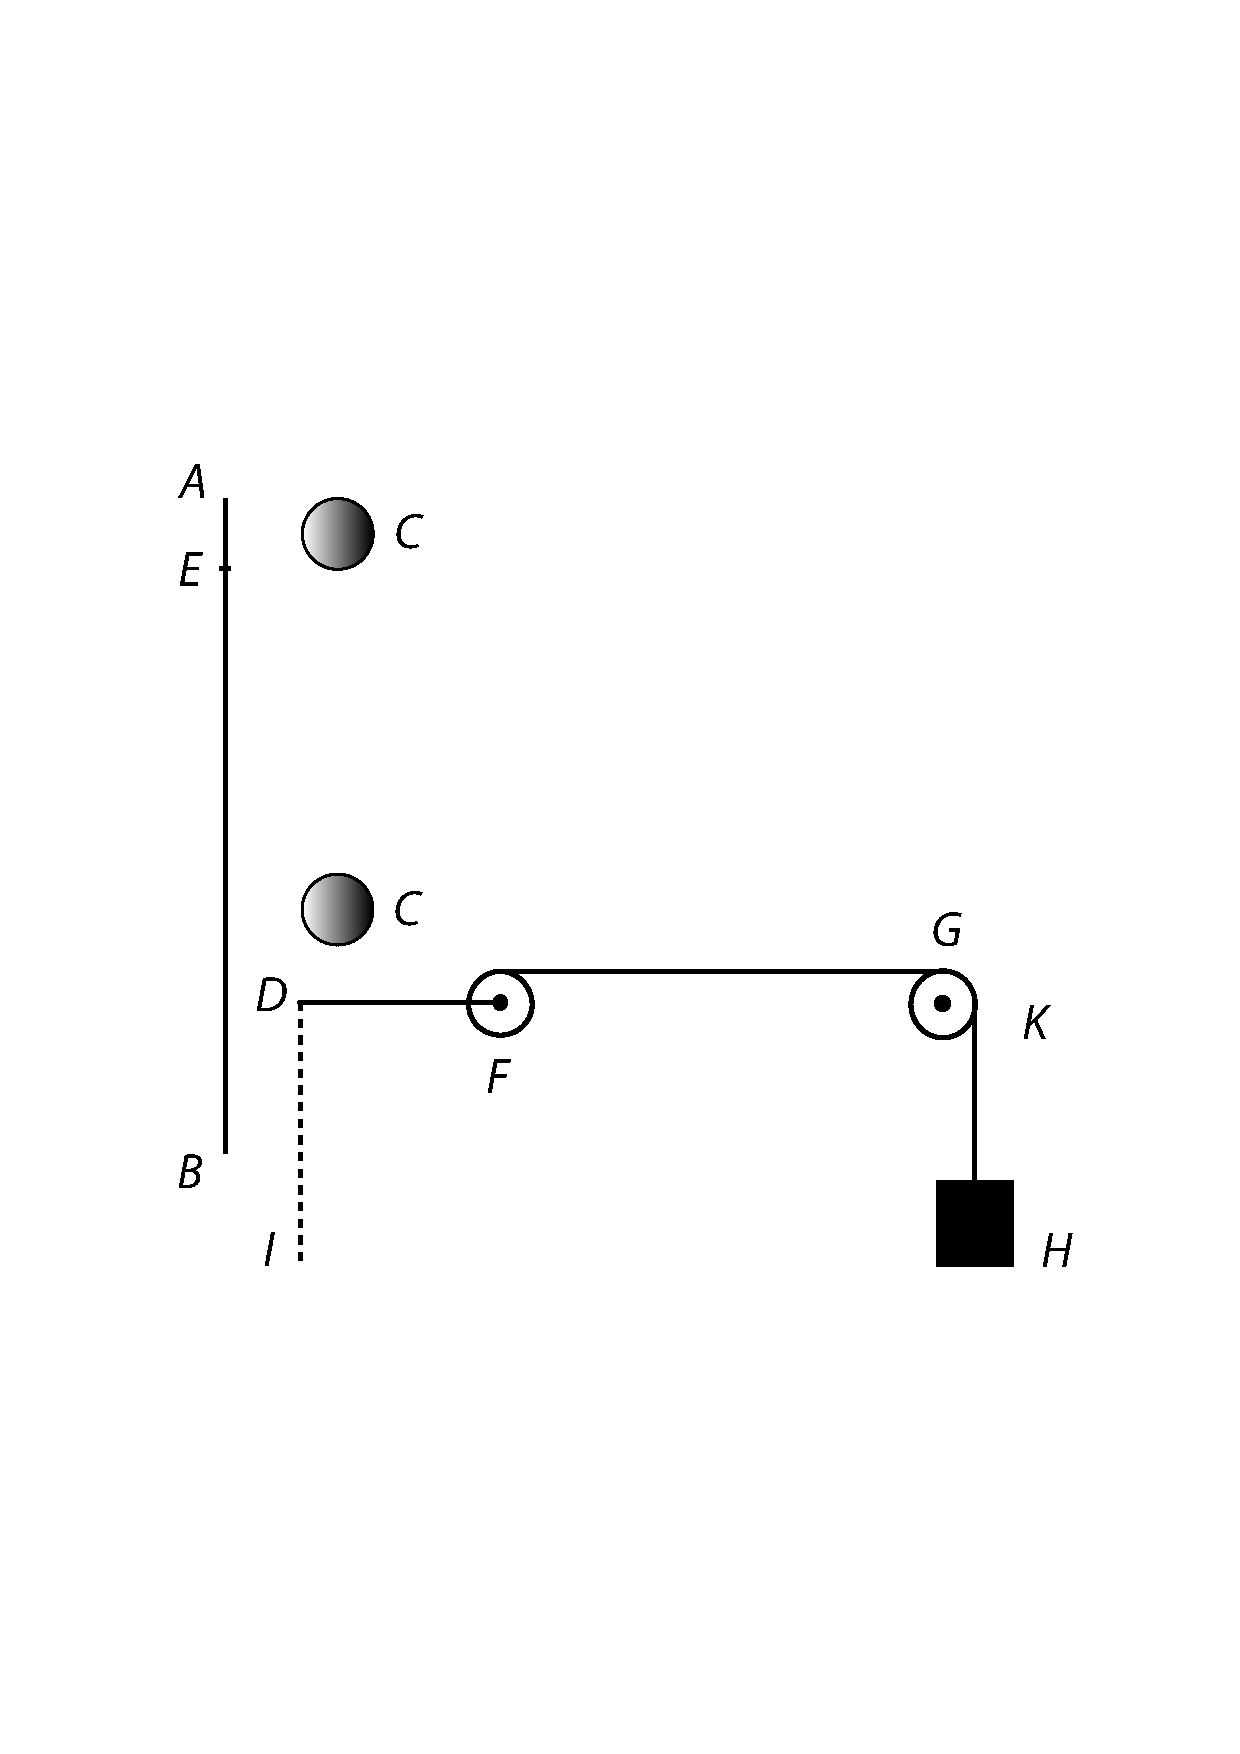
\includegraphics[trim = 30mm 80mm 18mm 74mm, clip, width=0.46\textwidth]{images/lh03705_008-d1.pdf}\\
%\noindent \centering [\textit{Fig. 4}] 
%\end{wrapfigure}
Credebam me naturam ictus plene tenere, sed nunc neque me, neque alios in ea re satisfecisse invenio.\edlabel{LH037,05_5v+8r_2} Esto linea \edtext{\textit{AB}, repraesentans tempus quo}{\lemma{\textit{AB},}\Bfootnote{\textit{(1)}\ in qua \textit{(2)}\ repraesentans [...] quo \textit{L}}} descendat corpus \textit{C}. Primo momento agat nisu primo, qui sit instar lineae \textit{AE} infinite parvae, seu incipiat \edtext{moveri,}{\lemma{}\Bfootnote{moveri,  \textbar\ seu eo momento aget \textit{ gestr.}\ \textbar\ et \textit{L}}} et quia quolibet momento tantundem novi impetus\protect\index{Sachverzeichnis}{impetus} accipit, ideo impetus in fine temporis \textit{B} erit ad impetum\protect\index{Sachverzeichnis}{impetus} primum, ut linea \textit{AB} ad lineam \textit{AE} seu ad punctum. Ictum\protect\index{Sachverzeichnis}{ictus} ergo quem inferet \edtext{Galilaeus\protect\index{Namensregister}{\textso{Galilei} (Galilaeus, Galileus), Galileo 1564-1642}}%
{\lemma{Galilaeus}\Cfootnote{\cite{01091}G. \textsc{Galilei}, \textit{Les mechaniques}, Paris 1634, S. 69-73.
Siehe dazu oben, N.~9.}} et post eum, qui rem magnam demonstrasse sibi in eo visus est \edtext{Borellus,\protect\index{Namensregister}{\textso{Borelli} (Borellus), Giovanni Alfonso 1608-1679}}%
{\lemma{Borellus}\Cfootnote{\cite{01001}G. A. \textsc{Borelli}, \textit{De vi percussionis}, Bologna 1667, cap. XXVII-XXIX (S. 192-210).}} ajunt esse infinitum. Ego vero ajo celeritatem\protect\index{Sachverzeichnis}{celeritas} esse infinitam, vires\protect\index{Sachverzeichnis}{vis} seu ictum\protect\index{Sachverzeichnis}{ictus} quem inferat non esse, nec ex \edtext{illa Hypothesi explicari}{\lemma{illa}\Bfootnote{\textit{(1)}\ ratione ex \textit{(2)}\ Hypothesi explicari \textit{L}}} posse, cur \edtext{corpus}{\lemma{}\Bfootnote{corpus  \textbar\ acceleratum \textit{gestr.}\ \textbar\ fortius \textit{L}}} fortius agat, quando altius lapsum etsi explicari possit celeritas motus. Quod ita demonstro. Cogitetur impingere corpus \textit{C} in dentem\protect\index{Sachverzeichnis}{dens} \textit{DF}, ex trochlea\protect\index{Sachverzeichnis}{trochlea} \textit{F} exeuntem, atque ita circumacta trochlea\protect\index{Sachverzeichnis}{trochlea} \textit{F} circumagi et trochleam\protect\index{Sachverzeichnis}{trochlea} \textit{G} intercedente fune\protect\index{Sachverzeichnis}{funis} \textit{FGH}, atque ita et elevari pondus\protect\index{Sachverzeichnis}{pondus} \textit{H}. Jam \edtext{pone corpus}{\lemma{pone}\Bfootnote{\textit{(1)}\ celeritatem\protect\index{Sachverzeichnis}{celeritas} corporis \textit{(2)}\ corpus \textit{L}}}\hfill \textit{H}\hfill esse\hfill gravius\hfill corpore\hfill \textit{C},\hfill et\hfill tamen,\hfill ut\hfill experientia\hfill docet\hfill ab\hfill eo\hfill attolli,\hfill utique\hfill si
\pend
\newpage
\pstart
%\begin{wrapfigure}[13]{l}{0.46\textwidth}
%\vspace{-11pt}
\centering 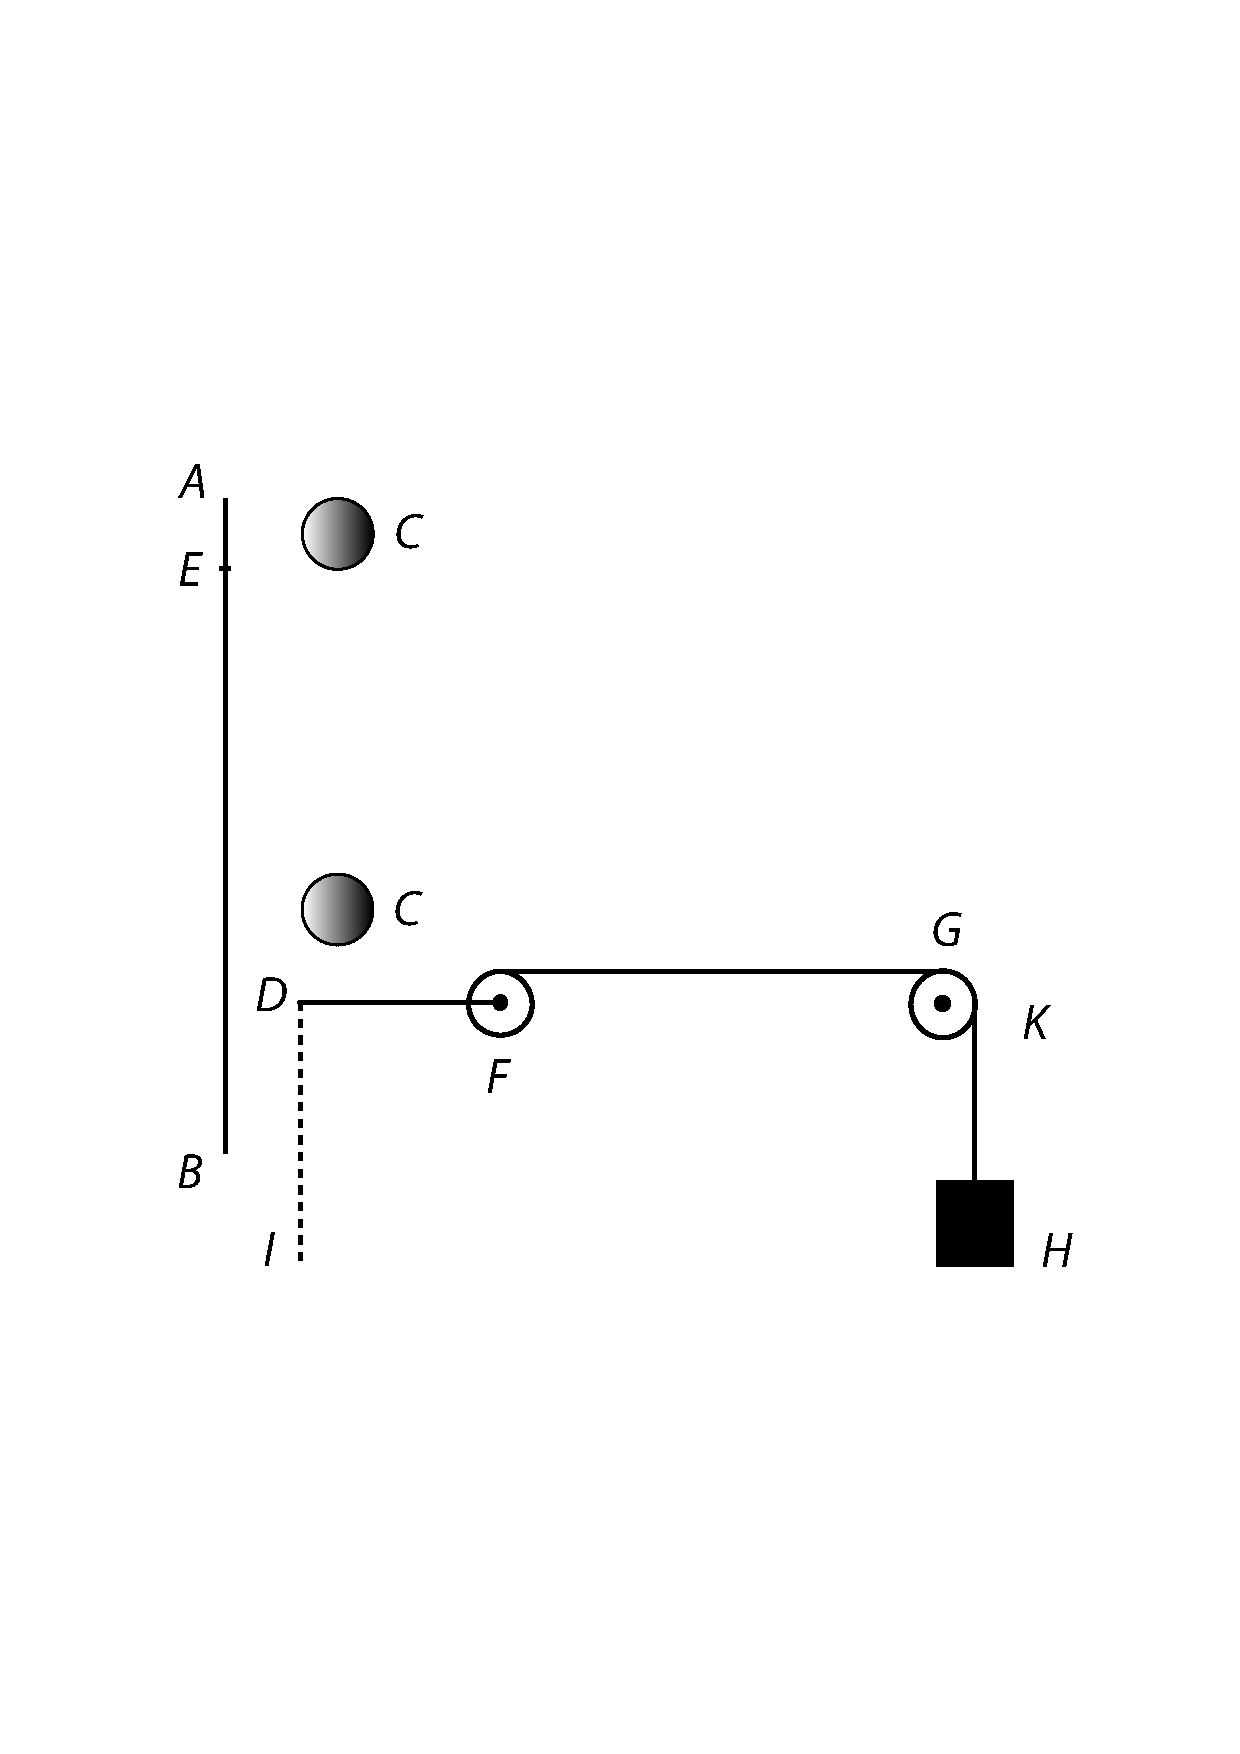
\includegraphics[trim = 0mm -3mm 0mm 0mm, clip, width=0.46\textwidth]{images/lh03705_008-d1.pdf}\\
\noindent \centering [\textit{Fig. 4}] 
%\end{wrapfigure}
\pend
\vspace{1.5em}
\pstart \noindent ea,\setline{1} quam retuli hypothesis vera est, id tribuendum est celeritati\protect\index{Sachverzeichnis}{celeritas} corporis \textit{C}, quae quod ejus ponderi deest compensat. Sed hic ecce incommodum ingens, \edtext{si post impactum corpus}{\lemma{si}\Bfootnote{\textit{(1)}\ natura co \textit{(2)}\ post [...] corpus \textit{L}}} \textit{C} descendit ad profunditatem quantulamcunque \textit{DI}, corpus \textit{H} ascendet ad aequalem ei, \textit{HK}. Absurdum autem est corpus aliquod \edtext{magis grave ascendere ut minus grave tantumdem}{\lemma{magis grave}\Bfootnote{%
\textit{(1)}\ tantum ascendere quantum necesse est \textit{(2)}\ ascendere [...] tantumdem \textit{L}}} descendat. Cum hac ratione natura agat contra seipsam. Non descendet ergo corpus \textit{C}, usque ad \textit{I}, id est non descendet omnino, nec ulla ratione attollet \textit{H}, cum \textit{DI} posita sit quantulacunque. Nondum ergo video cur corpus ab alto lapsum, aliud gravius \edtext{in aliquantulam}{\lemma{in}\Bfootnote{\textit{(1)}\ alio \textit{(2)}\ aliquantulam \textit{L}}} altitudinem \edtext{attollat. Sed huic objectioni respondetur, naturam magis deprimere corpus leve, sed fortiter conans, quam grave debiliter conans, quia non est gravitas, sed gravitatio seu conatus qui considerari debet. Quare concludo celeritatem motus non augere resistentiam ab attritu\protect\index{Sachverzeichnis}{attritus}.}{\lemma{attollat.}\Bfootnote{\textit{(1)}\ Necesse est ergo rem non a celeritate\protect\index{Sachverzeichnis}{celeritas} corporis aucta, etsi aucta sit, sed ab aucto \textit{(2)}\ Sed [...] attritu. \textit{L}}}
\pend 
\pstart
   Redeo jam ad \edtext{contemplationem corporum quae aliis innituntur, propellendorum.
Ponamus in plano horizonti parallelo \textit{BC} esse}{\lemma{contemplationem}\Bfootnote{%
\textit{(1)}\ rotarum circumvolvendarum %
\textit{(2)}\ corporum [...] propellendorum. %
\textit{(a)}\ Ea ponamus in plano esse %
\textit{(b)}\ Ponamus [...] esse \textit{L}}} corpus \textit{A}. Id impellenti resistet
% \begin{wrapfigure}[12]{l}{0.49\textwidth}
%\vspace{-2mm}
%   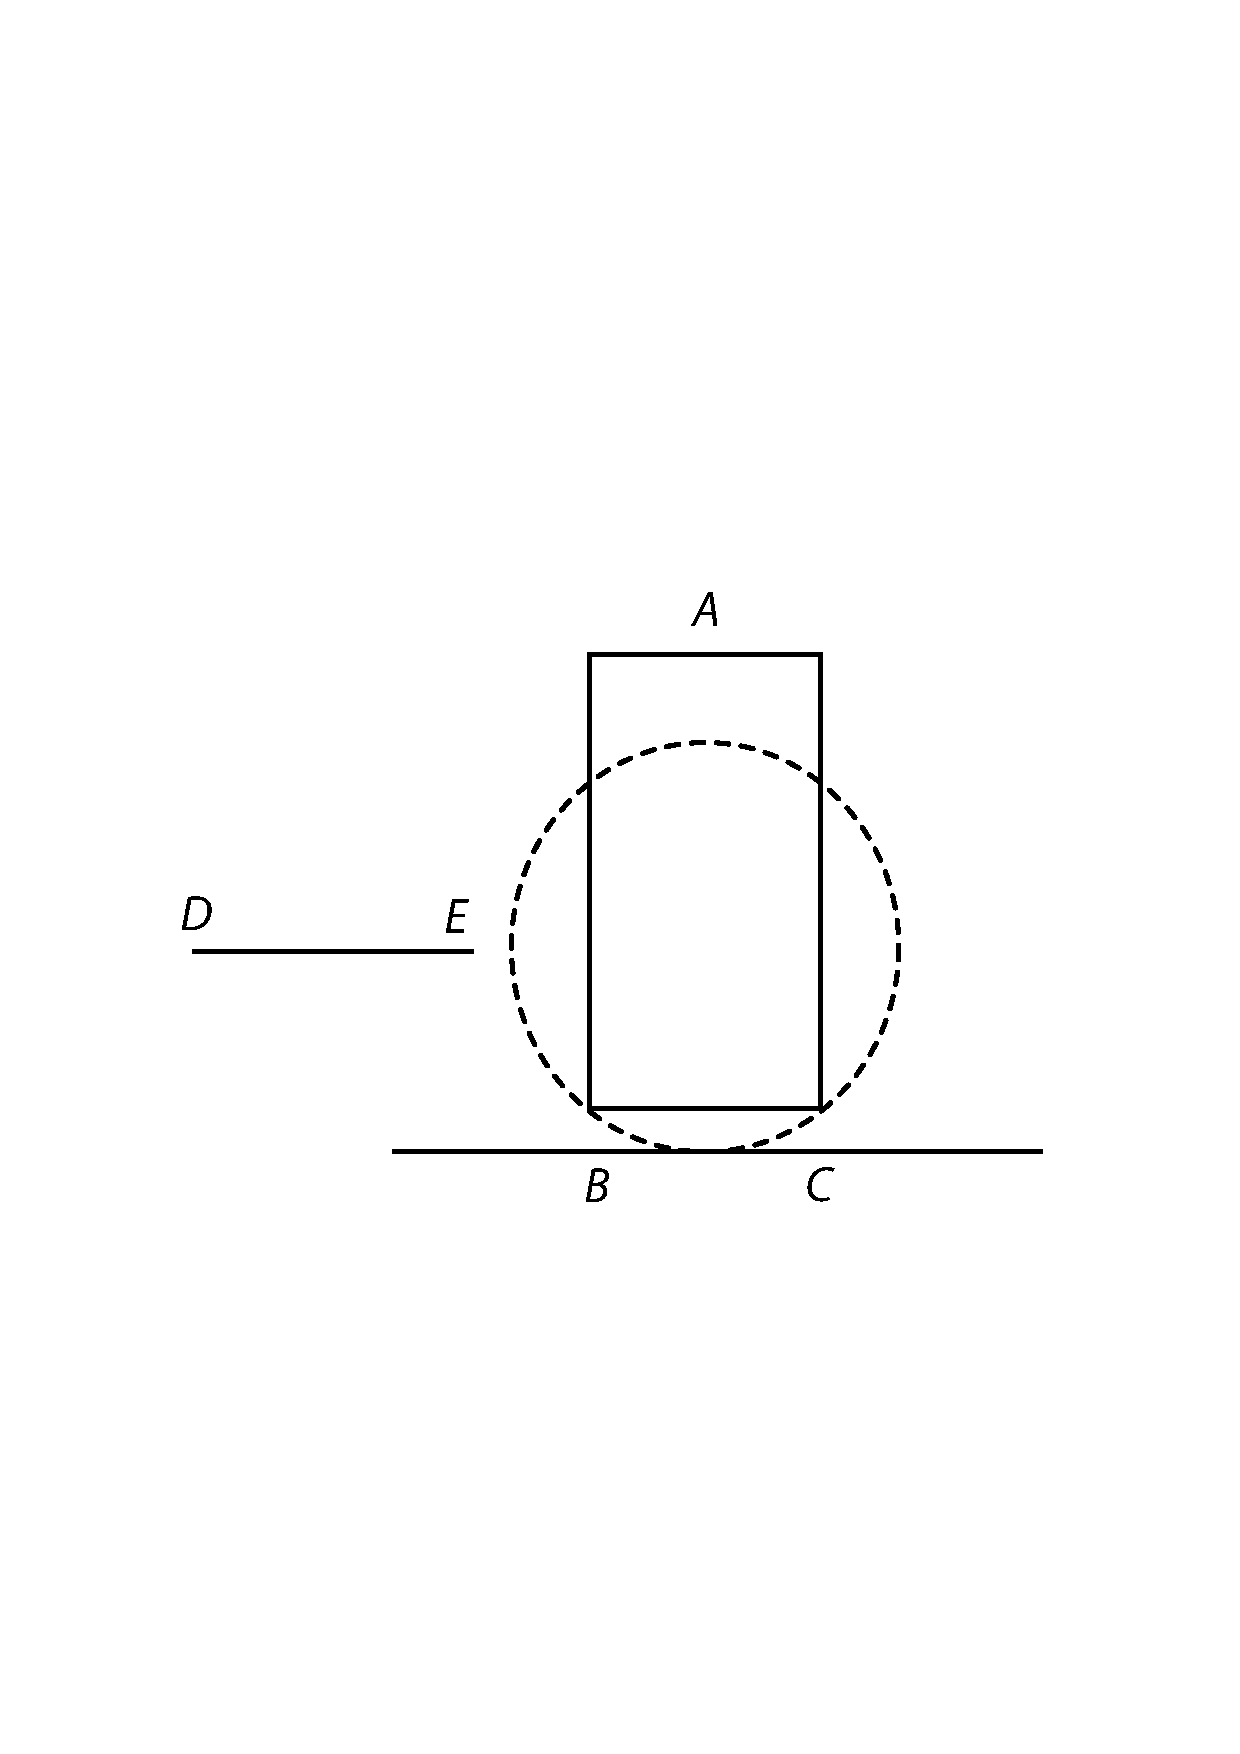
\includegraphics[trim = 28mm 88mm 24mm 100mm, clip, width=0.49\textwidth]{images/lh03705_008-d2.pdf}
%\noindent \centering [\textit{Fig. 5}] 
%    % \caption{Bildbeschreibung}
%    \end{wrapfigure}
attritu, qui a plani \textit{BC} scabritie oritur, nec impelli potest, nisi vel abrasis resistentibus vel inflexis, vel \edtext{superatis. Si}{\lemma{superatis.}\Bfootnote{\textit{(1)}\ Pone jam impelli \textit{(2)}\ Si \textit{L}}} abradenda sunt patet variari difficultatem pro corporis plani friabilitate;
\pend
\newpage
\pstart
\centering
 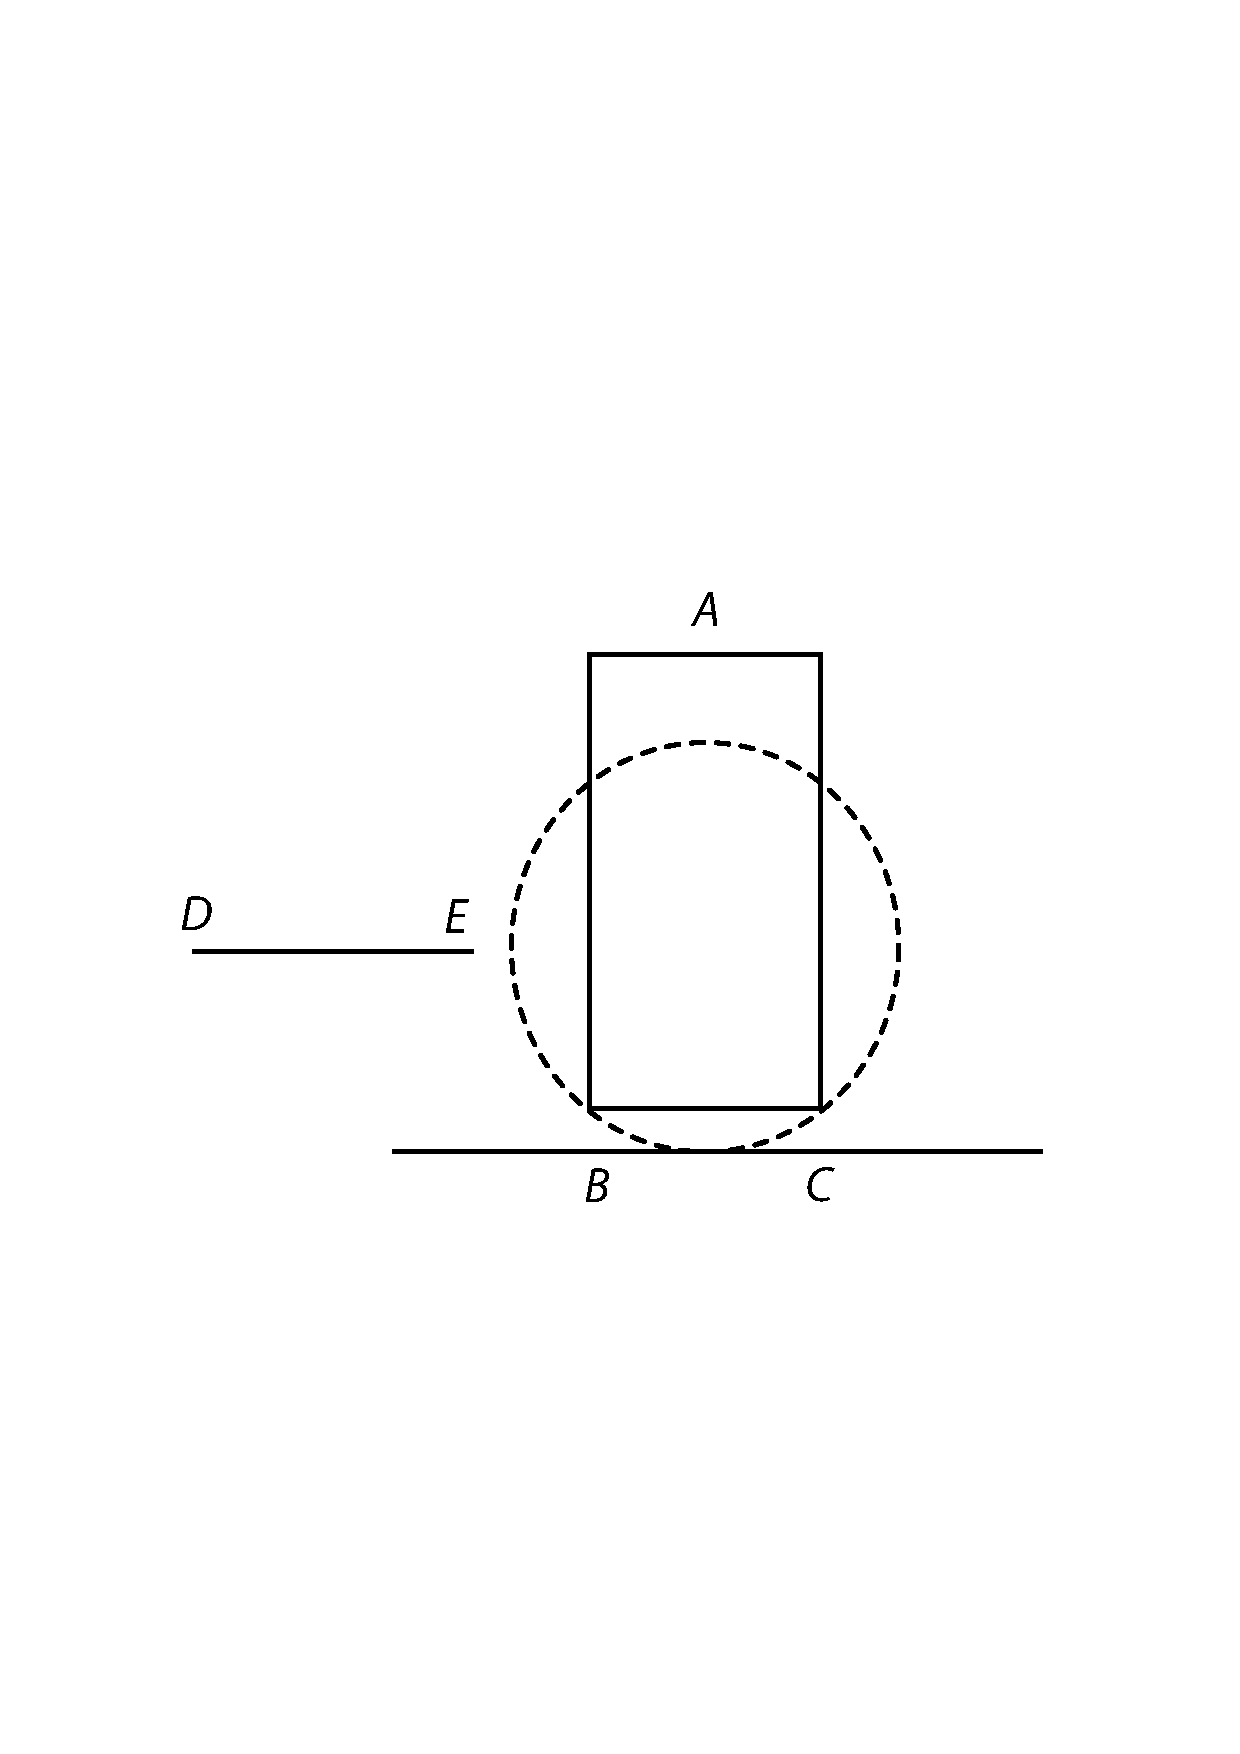
\includegraphics[trim = 0mm 0mm 0mm 0mm, clip, width=0.49\textwidth]{images/lh03705_008-d2.pdf}\\
\noindent \centering [\textit{Fig. 5}] 
%    % \caption{Bildbeschreibung}
\pend
\vspace{1.5em}
\pstart \noindent si \setline{1}inflectenda pro duritie, si superanda pro inaequalitate. Sed cum ista infinitas contineant varietates, ideo ut ad calculum res queat revocari facilius, considerabimus attritum ut uniformem quandam causam, quae motum impediat, instar glutinis cujusdam, aut infinitorum in omnibus punctis ponderum \edtext{appensorum. [8~v\textsuperscript{o}]\\
\hspace*{7,5mm}Jam ponamus}{\lemma{appensorum.}\Bfootnote{\textit{(1)}\ Quibus ita positis \textit{(2)}\ Jam ponamus \textit{L}}}
corpus \textit{A}, impelli linea \textit{DE}.
\edtext{Alibi}{\lemma{Alibi}\Cfootnote{Stelle nicht nachgewiesen. Siehe aber \cite{01156}\textit{LSB} VI, 2 N.~42\textsubscript{4}, S.~281.16-18.}}
autem a me ostensum est in linea qualibet alias omnes contineri, ideo qui impellit in linea \textit{DE}, is etiam impellere putandus est in linea circulari \textit{EG}, quae centro \textit{F}, radio \textit{FE}, describitur. Et ex omnibus lineis possibilibus, quibus impulsus\protect\index{Sachverzeichnis}{impulsus} cogitari potest fieri, ea eligetur, qua facillime exitum sortitur impulsus\protect\index{Sachverzeichnis}{impulsus}, quia ex omnibus punctis lineae \textit{HF}, remotissimum a puncto impactus \textit{E} est punctum \textit{F}, ideo maximus etiam radius \textit{FE}, at maximo radio, major motus, seu facilior exitus. Haec causa est cur corpora, \edtext{quae nonnihil excelsa, atque excelso loco}{\lemma{quae}\Bfootnote{\textit{(1)}\ alto sa \textit{(2)}\  nonnihil [...] loco \textit{L}}} impulsa, facilius evertantur quam propellantur, caeterum quanto minor est [\textit{HF}]\edtext{}{\Bfootnote{\textit{EH}\textit{\ \ L \"{a}ndert Hrsg.}}} et major [\textit{EH}]\edtext{}{\Bfootnote{\textit{HF}\textit{\ \ L \"{a}ndert Hrsg.}}} tanto facilior eversio est; cujus rei ratio est, quod quanto \textit{HF} longior est, tanto magis corpus ponderat in \textit{H}, tantoque difficilius elevatur, quod tamen ad eversionem necesse est. 
%\begin{wrapfigure}[13]{l}{0.48\textwidth}
%\vspace{-4pt}
%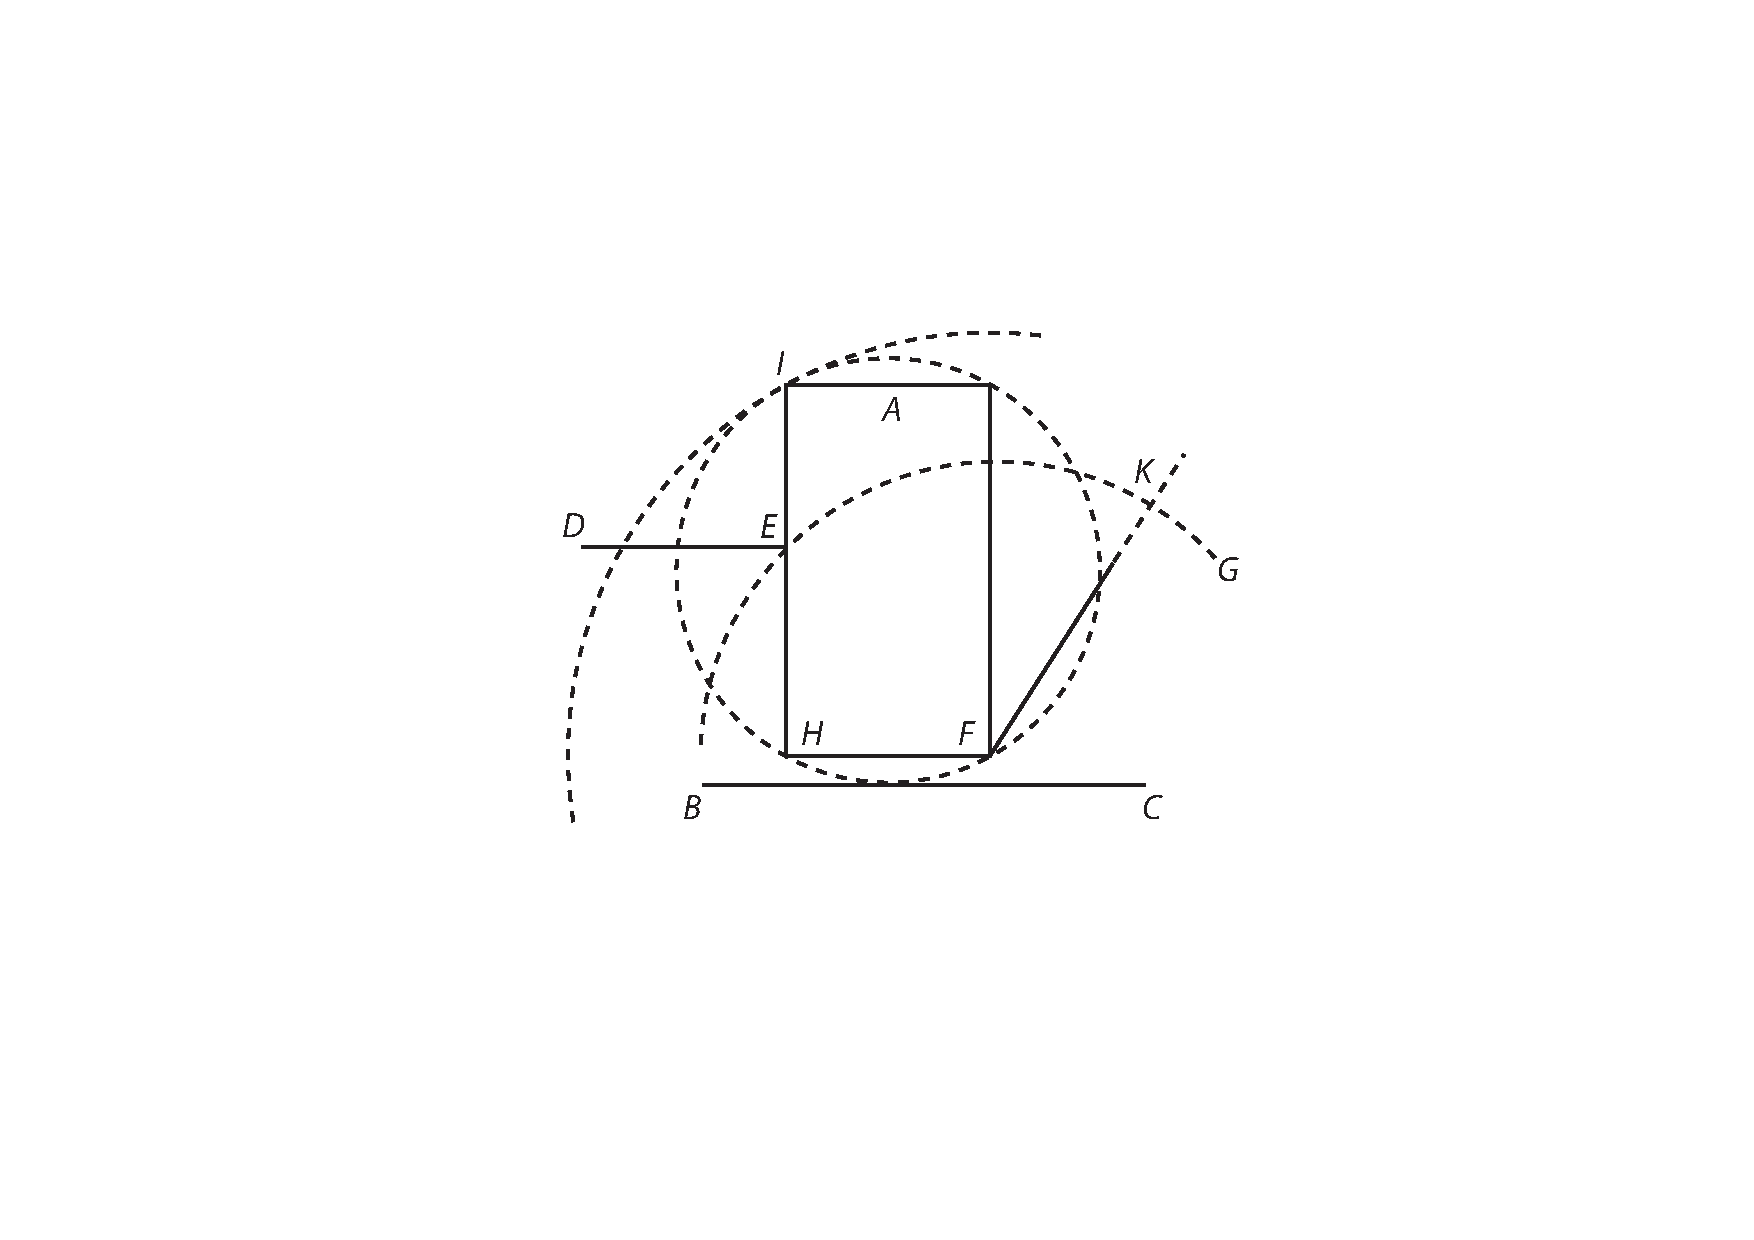
\includegraphics[trim = 0mm 0mm 0mm 0mm, clip, width=0.48\textwidth]{images/lh03705_008-d3.pdf}\\
%\noindent \centering [\textit{Fig. 6}] 
%\end{wrapfigure}
\edtext{Conferenda gravitas\protect\index{Sachverzeichnis}{gravitas}}{\lemma{}\Bfootnote{Conferenda  \textbar\ ergo \textit{gestr.}\ \textbar\ gravitas \textit{L}}}
\edtext{corporis in \textit{H}}{\lemma{corporis}\Bfootnote{\textit{(1)}\ ex \textit{H} \textit{(2)}\ in \textit{H} \textit{L}}} ex centro \textit{F}, cum attritu\protect\index{Sachverzeichnis}{attritus} [ipsius]\edtext{}{\Bfootnote{ipso\textit{\ \ L \"{a}ndert Hrsg.}}} \textit{HF}. \edtext{Ergo si}{\lemma{Ergo}\Bfootnote{\textit{(1)}\ quanto \textit{(2)}\ si \textit{L}}} [\textit{HF}]\edtext{}{\Bfootnote{\textit{HI}\textit{\ \ L \"{a}ndert Hrsg.}}} brevis, corpus facilius evertetur et si attactus parum versus \textit{H}, multum versus \textit{F}. Sed [haec]\edtext{}{\Bfootnote{hae\textit{\ \ L \"{a}ndert Hrsg.}}} facilia, corpus eversum ponatur in aliam quandam faciem \textit{FK}, qualis fuit \textit{HF}, pro-
\pend
\newpage
\pstart
\centering
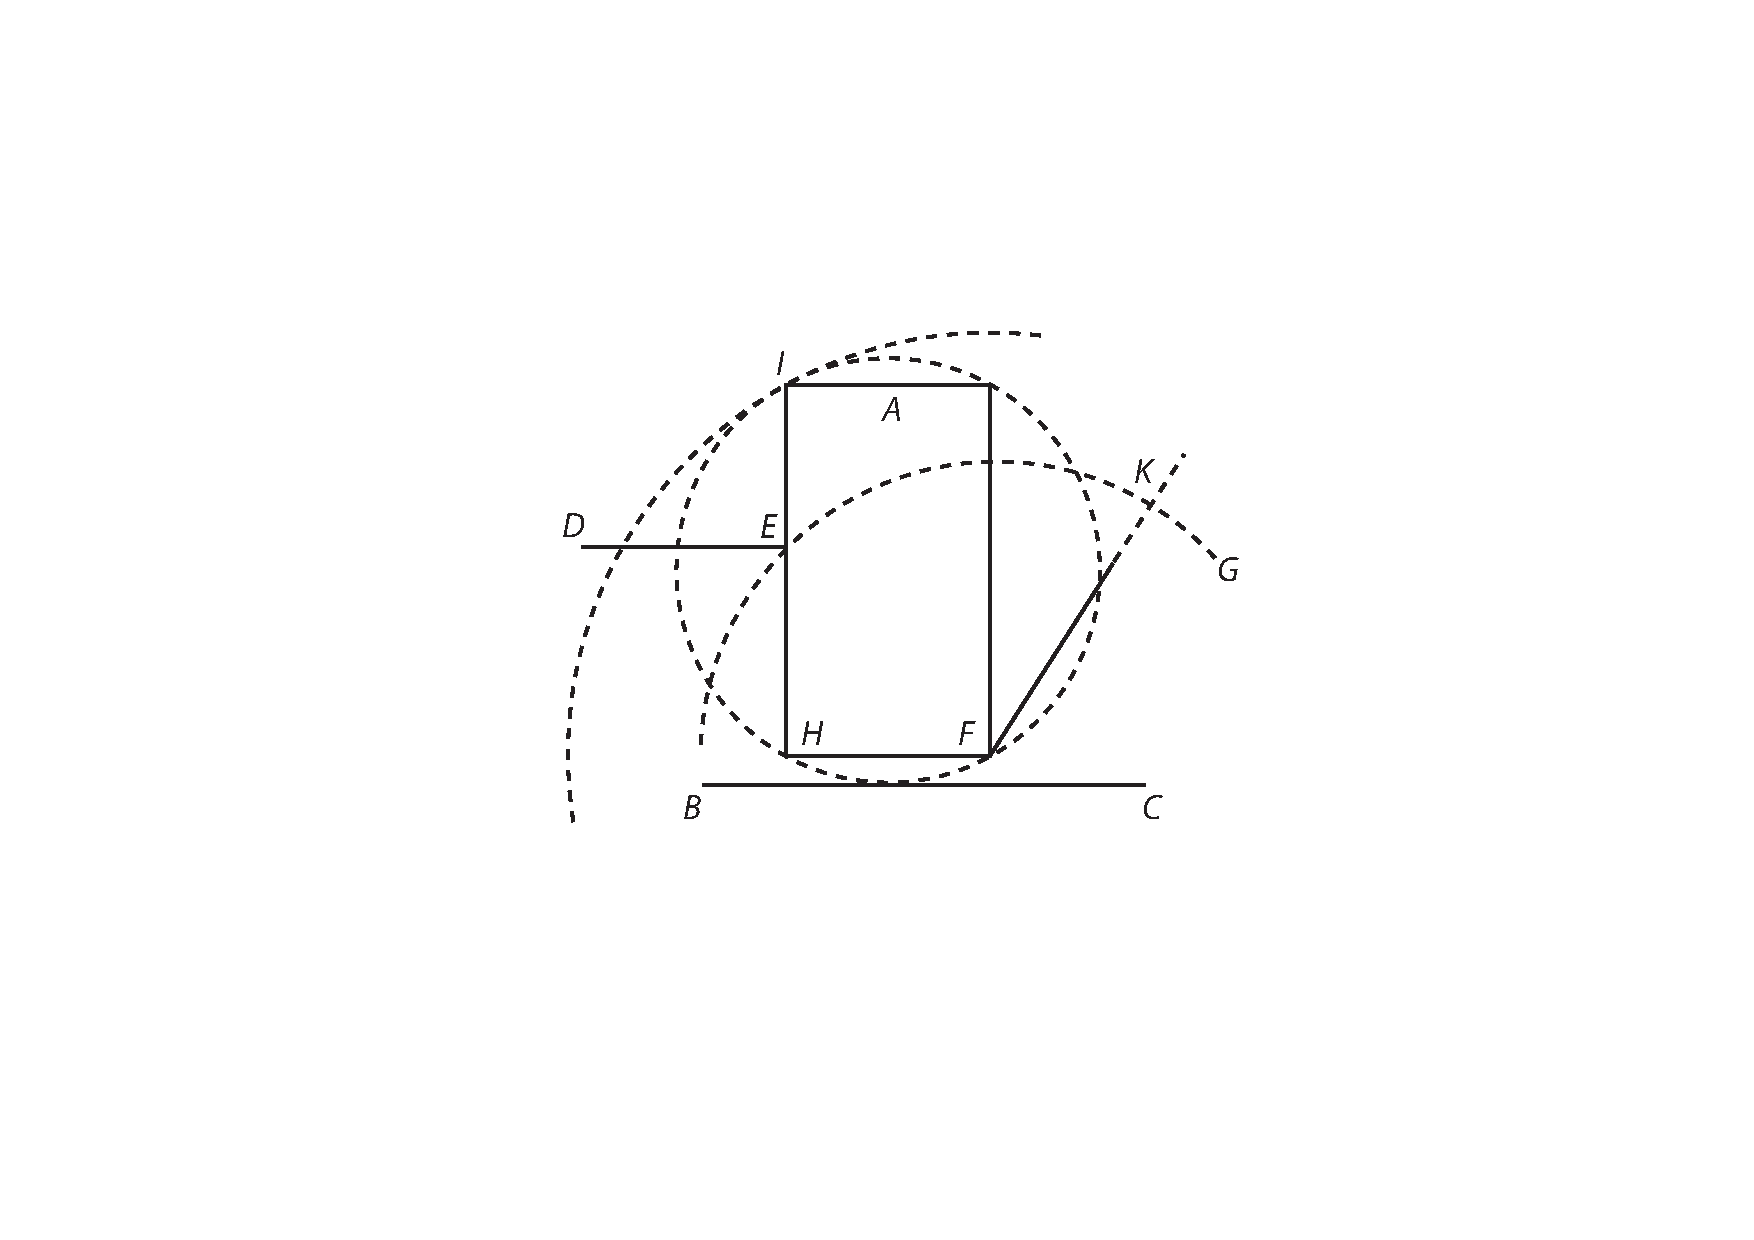
\includegraphics[trim = 0mm -2mm 0mm 0mm, clip, width=0.52\textwidth]{images/lh03705_008-d3.pdf}\\
\noindent \centering [\textit{Fig. 6}] 
\pend
\vspace{1.5em}
\pstart \noindent cedere,\setline{1} ac denique ipsas \textit{HF}, et \textit{FK}, esse admodum parvas atque sic satis uniformes, habebimus id quod rotam vulgo appellamus, in quo linea \textit{HF} valde \edtext{parva, \textit{EH}}{\lemma{parva,}\Bfootnote{\textit{(1)}\ \textit{AK} \textit{ (2) }\ \textit{EH} \textit{L}}} infinities major, ideoque eversio facillima, et continuo repetenda ob figurae in se recurrentis uniformitatem. Manifestum est autem huic eversionis motui attritum\protect\index{Sachverzeichnis}{attritus} non obstare, neque aut raptura flexuque partium scabrarum, neque subsultatione corporis ad eas separandas opus esse. Hinc jam colligitur quanto rotae sunt majores tanto esse utiliores, eo enim major est linea \textit{FE}.
\pend 
\pstart
   Hinc colligo si currus non [centris]\edtext{}{\Bfootnote{centris,\textit{\ \ L \"{a}ndert Hrsg.}}} rotarum inniteretur, sed tangentis more ipsi circumferentiae incumberet, celerius iturum. Sed rationem habuisse homines, quod centris incumbere maluerunt, quia ita eadem rota perpetuo servit, at posteriore modo continua rotarum serie ad currum perpetuo sustinendum opus foret aut arte, qua rota
%\begin{wrapfigure}[11]{l}{0.4\textwidth}
%%   \vspace{-22mm}
% \includegraphics[trim = 0mm 0mm 0mm 0mm, clip, width=0.4\textwidth]{images/lh03705_008-d4.pdf}\\
%\noindent \centering [\textit{Fig. 7}] 
%%    % \caption{Bildbeschreibung}
%   \end{wrapfigure}
deserta seu posterior subito inter priores \edtext{collocaretur. Nec credo}{\lemma{collocaretur}\Bfootnote{\textit{(1)}\ , quod nescio an \textit{(2)}\ . Nec credo \textit{L}}} lucrum fore tantum, ut incommoditatem sit pensaturum. Cur rotae \edtext{radios}{\lemma{}\Bfootnote{radios \textit{erg.} \textit{L}}} habeant, non solidae sint orbium instar ratio est, ut quantum poterat, salva firmitate de pondere detraheretur. Patet quoque\setline{11} cur vietores,
\pend
\vspace{1.2em}
\pstart
\noindent\centering
\includegraphics[trim = 0mm -3mm -5mm 0mm, clip, width=0.35\textwidth]{images/lh03705_008-d4.pdf}\\
\noindent \centering [\textit{Fig. 7}] 
\pend 
\count\Bfootins=1200
\pstart
\begin{wrapfigure}[5]{l}{0.38\textwidth}
 \vspace{-5mm}
\includegraphics[trim = 0mm -3mm 0mm 0mm, clip, width=0.38\textwidth]{images/lh03705_008-d5.pdf}\\
\noindent \centering [\textit{Fig. 8}] 
%    % \caption{Bildbeschreibung}
 \end{wrapfigure}
\noindent (les Tonneliers) tonnas sive vasa lignea facilius per plateas provolvant, quam portent, etsi enim attritus\protect\index{Sachverzeichnis}{attritus} obstet provolventi, non obstet portanti, tamen portans onus sustinet, quod cum provolvis sustinet terra. Attritus\protect\index{Sachverzeichnis}{attritus} autem valde diminutus est, ope rotae.\\
\indent Minueretur adhuc amplius attritus\protect\index{Sachverzeichnis}{attritus}, si currus non inaequalibus plateis aut etiam profunda terra limoque, sed tabulis planis, irent, quem in finem fieri posset, ut Tabulae se perpetuo substernerent rotis, aliae atque aliae, atque invicem redeuntes. % PR: getilgte FN: \edtext{}{\lemma{redeuntes}\Cfootnote{M\"{o}glicherweise bezeichnet in [\textit{Fig. 8}] der erste Kreis von links ein einfaches Rad, der mittlere ein auf einer flachen Platte rollendes Rad, der letzte ein im Schlamm rollendes Rad.}}
Quod et nonnullos non infeliciter molitos intelligo. % PR: getilgte FN: \edtext{}{\lemma{intelligo}\Cfootnote{???? Anspielung auf ????.}} 
[9~r\textsuperscript{o}]
\pend 
\count\Bfootins=1100
\count\Cfootins=1100
\pstart